% MATHS DIWALI ASSIGNMENT 

% Kavit Kheni 
% 201701409

\documentclass[12pt]{article}
\usepackage{graphicx}
\usepackage{times}

\usepackage[utf8]{inputenc}
\usepackage[english]{babel}
 
\usepackage[nottoc]{tocbibind}

\usepackage{type1cm}
\usepackage{eso-pic}

\usepackage{color}
\usepackage{ulem}
\usepackage{everypage}
\usepackage{amssymb}
%\usepackage{draftwatermark}
% Use the following to make modification
\usepackage[margin=3 cm]{geometry}
%packages added
\usepackage{amsmath}

%\usepackage[usenames,dvipsnames]{color}
\begin{document}

%\SetWatermarkAngle{45}
%\SetWatermarkText{KAVIT KHENI}
%\SetWatermarkScale{0.5}
%\SetWatermarkAngle{45}
%\SetWatermarkLightness{0.95} 
%\SetWatermarkFontSize{1cm}
%\SetWatermarkScale{5}
%\SetWatermarkText{Kavit Kheni}


% Article top matter
\title{\textcolor{red}{Calculus used in CHEMICAL KINETICS}}

\begin{center}
\Huge
{\bf \textcolor{blue}
{ 
{How mathematics is develop...} \\
}
}
\vspace{2 cm}
\huge\bf
{ Assigned by : Professor Manish K. Gupta \\
COURSE : SC 107 \\
{\bf \textcolor{red}
{
{Chemistry With Calculus} \\
}
FALL 2017 \\
DA-IICT \\
GANDHINAGAR \\
}
\vspace{6 cm}
\LARGE {\it
{ 
Made by: Kavit Kheni \\
ID : 201701409 \\
Email ID : kavit3010@gmail.com\\
}
}
}
\end{center}

\author{
Kavit Kheni\\
201701409,\\
DA-IICT,\\
GANDHINAGAR,\\
INDIA\\
\texttt{201701409@daiict.ac.in}
} 
\date{\today}
%\today is replaced with the current date

\maketitle
\begin{abstract}
\textcolor{blue}
{
\large
{
     We thought that how mathematics is develop and why mathematics is important. So that in this project, I discuss how to use calculus for chemical reaction. I will discuss how differential equation  of calculus played an important role for determining the rate law of chemical reactions.
		And we also predict that after how much time the "EARTH" will destroy due to depletion in OZONE layer by the help of calculus.
}
}
\end{abstract}




\begin{figure}[h!]
\centering

\includegraphics[scale=3]{DA-IICT.jpg}
%%\caption{My test image}
\end{figure}

\newpage
\large
\section{\textcolor{red}{PREFACE}}
Chemical reactions convert substances with well-defined properties into other materials with different properties. Chemical kinetics is the study and discussion of chemical reactions with respect to reaction rates, effect of various variables, re-arrangement of atoms, formation of intermediates etc.Chemical kinetics, also known as reaction kinetics. Chemical reaction rates are the rates of change in concentrations or amounts of either reactants or products. For changes in amounts, the units can be one of mol/s, g/s, lb/s, kg/day etc. For changes in concentrations, the units can be one of mol/(L s), g/(L s), /s etc.
        Determining rates of chemical reactions is a crucial first step in the design of any commercial chemical process, so this is an area of particular interest to chemists and chemical engineers.   

\section{\textcolor{red}{ MATHEMATICAL MODEL }}
\textsf
A mathematical model for rate at which we will get product with respect to time. From Experimental results,it was found that chemical rate equation is in the form of differential equation.
For that generalized equation is derived below. 
\subsection{\textcolor{blue}{n th order chemical reaction}}
{
For some reaction {A  \rightarrow  B  +  C},
$At the time of initialization of process, quantity of B an C is null and suppose quantity of A is 'a'.$
\\$After some time 't', B and C will be produced by quantity suppose 'x', so quantity of A will be 'a-x'.$ 
}

$$\textcolor{blue}{r=k{(a-x)}^{n}}\_\_\_\_\_\_\_\_\_\_(1)$$
where r is rate of the reaction.k is rate constant. n is order of the reaction.(a-x) is concentration of A at any time t.
\\This equation says that rate of reaction 'r' is directly proportional to concentration of A to the power n.
\\$$  \textcolor{blue}{r=-\frac{d\,[A]}{dt}=+\frac{d\,[B]}{dt}=+\frac{d\,[C]}{dt}}\_\_\_\_\_\_\_\_\_\_(2)$$
\\Where rate of reaction = (Instantiation rate of disappearance of A) = +(Instantiation rate of appearance of B or C)
\\Now, by equating equation (1) and (2)
$$ \textcolor{blue}{k{(a-x)}^{n}=+\frac{d\,[B]}{dt}}$$
The concentration of B after time t is x.
$$  \textcolor{blue}{k{(a-x)}^{n}=+\frac{d\,x}{dt}}$$
By integrating both the side,
$$ \textcolor{blue}{\int_{0}^{x}{\frac{d\,x}{{(a-x)}^{n}}}=\int_{0}^{t}{k\,dt}}$$
$$  \textcolor{blue}{\int_{0}^{x}{{(a-x)}^{-n}{d\,x}}=\int_{0}^{t}{k\,dt}}$$
$$  \textcolor{blue}{\frac{1}{n-1}[\frac{1}{{(a-x)}^{n-1}}-\frac{1}{{a}^{n-1}}]=kt}\_\_\_\_\_\_\_\_(3)$$
Where n = 0,2,3,4,5%...
\\n\neq1
\\\\{\color{red}{\textbf{Half Life}}}
\\ $ Definition : The time required for the conversion of reactant up to half of its initial concentration.$

$$\frac{1}{n-1}[\frac{1}{{(\frac{a_0}{2})}^{n-1}}-\frac{1}{{(a_0)}^{n-1}}]=kt$$
\\ $$kt_\frac{1}{2} = \frac{1}{n-1}[\frac{{2}^{n-1}-1}{({a_0)}^{n-1}}]\_\_\_\_\_\_\_\_\_\_(4)$$
\\$$t_\frac{1}{2}\propto \frac{1}{{(c_0)}^{n-1}}$$

\subsection{\textcolor{blue}{For Zero order reaction}}

from equation (3) we take n=0;
$$\frac{1}{n-1}[\frac{1}{{(a-x)}^{n-1}}-\frac{1}{{a}^{n-1}}]=kt\_\_\_\_\_\_\_\_(3)$$
$$x = kt$$
\\ where x is concentration of product which is also equal to ${c_0} - {c_t}.$

$$c_0 - c_t = kt$$
For half life 
\\$$c_t = \frac{c_0}{2}$$
\ $$t_\frac{1}{2} = \frac{c_0}{2k}$$

\subsection{\textcolor{blue}{For first order reaction}}
\begin{figure}[h!]
\centering
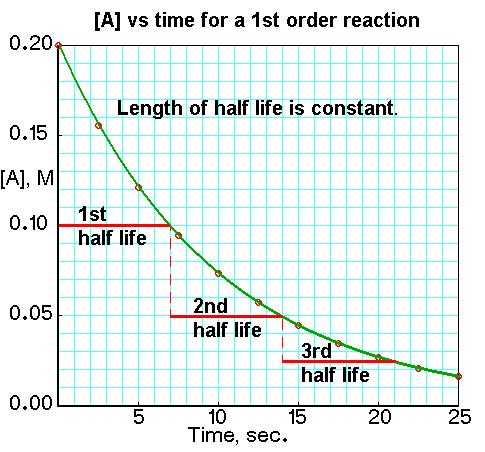
\includegraphics[scale=0.5]{first order.jpg}
%%\caption{My test image}
\end{figure}

\ We can not put n = 1 in equation (3) so,
\textcolor{black}{$$ \frac{d\,[A]}{dt}=-k\,[A]$$
\ $$\int{\frac{d\,[A]}{[A]}}=\int{-k\,dt}$$
\ $$log{|[A]|}=-kt+\kappa$$
\ $$[A]=-e^{-kt}e^{\kappa}$$
\ $$[A]=-\kappa\,e^{kt}$$}}
\ If we put limit then we will get,
$$ln{c_0} - ln{c_t} = kt$$
$$ c_t = c_0{e}^{-kt}$$
\\And half life of first order reaction is,
$$t_\frac{1}{2} = \frac{ln(2)}{k}$$
\\For first order reaction,
$$c_t=c_0(\frac{1}{2})^{n}
$$where n is number of half life.

\subsection{\textcolor{blue}{For second order reaction}}
\  We put n = 2 in equation (3),
$$\frac{1}{n-1}[\frac{1}{{(a-x)}^{n-1}}-\frac{1}{{a}^{n-1}}]=kt\_\_\_\_\_\_\_\_(3)$$
$$\frac{1}{c_t} - \frac{1}{c_0} = kt$$
Where $c_t$ is concentration of A at time t and $c_0$ is initial concentration of A.

\ Half life for second order reaction we take n = 2 in equation 4,
\\ $$kt_\frac{1}{2} = \frac{1}{n-1}[\frac{{2}^{n-1}-1}{({a_0)}^{n-1}}]\_\_\_\_\_\_\_\_\_\_(4)$$
$$t_\frac{1}{2} = \frac{1}{c_0k}$$
$$t_\frac{1}{2} \propto \frac{1}{c_0}$$
\section{\textcolor{red}{APPLICATION}}

Chemical kinetics is majorly concerned with the speeds, or rates, of reactions. It is not only to understand how to determine the rates at which reactions occur, but also to consider the factors that control these rates. The rates of reactions span an enormous range, from those that are complete within fractions of seconds, such as certain explosions, to those that take thousands or even millions of years, such as the formation of diamonds or other minerals in Earth’s crust. 

Chemical kinetics is a subject of broad importance. It relates, for example, to how quickly a medicine is able to work, to whether the formation and depletion of ozone in the upper atmosphere are in balance, and to industrial problems such as the development of catalysts to synthesize new materials. For example, what factors determine how rapidly food spoils? How does one design a fast-setting material for dental fillings? What determines the rate at which steel rusts? What controls the rate at which fuel burns in an automobile engine? 


\section{\textcolor{red}{CONCLUSION}} 

Calculus can be used in determining the rate at which we will get final product. And also used to predict quantity of reactants needed to get required amount of product. So it will help to determine the cost of reactants and from that we will also determine the cost of final product.
         
\newpage

\cite{*}
\bibliographystyle{plain}
\bibliography{201701409.bib}


\fontsize{50}{50}\selectfont{THANK  YOU ....}
\end{document} 
%End of document.

